\chapter{Vergleich und Bewertung zwischen Open API 2.0 und Open API 3.0}
\label{cha:k6}
Ende 2016 wurde die Open API Specification 3.0 schließlich von der Open API Initiative veröffentlicht. Es ist eine Hauptversion und nach 3 Jahren hat es eine Menge Verbesserungen gegenüber der Open API 2.0-Spezifikation gebracht, sodass Definitionen für eine breitere Palette von APIs erstellt werden können. In diesem Kapitel werden die Hauptunterschiede zwischen Open API 2.0 und 3.0 nach der Quellen\cite{swagger20Github, openapi20Github} aufgezeigt.

\section{Strukturelle Verbesserungen}

Mit der OpenAPI Specification Version 3.0 wurde die Gesamtstruktur des Dokuments vereinfacht:

\newpage

\begin{figure}[h]
	\centering
	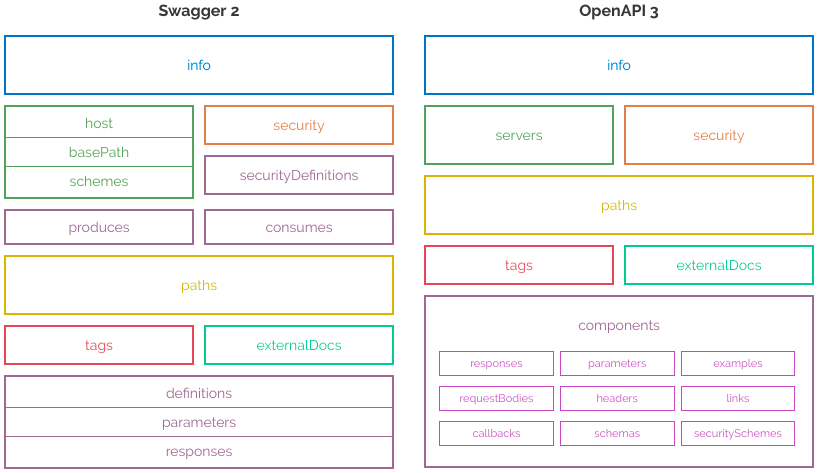
\includegraphics[width=10cm]{openapi2u3.png}
	\caption{Überblick über die Struktur der Open API 2.0 und Open API 3.0 Spezifikationen\cite{openapi2u317}}
	\label{openapi2u317-1}
\end{figure}

\subsection{Versionsbezeichner (engl. Version Identifier)}

Version ist eine beliebige Zeichenfolge, die die Version von API angibt\cite{openapiversion17}. In 2.0 spec gibt es eine Eigenschaft namens "`swagger"', die die Version der Spezifikation angibt, zum Beispiel:\\

\begin{LaTeXCode}[caption={Version von Swagger},captionpos=b, label=LaTeXCode:swagger2.0-1][numbers=none]
"swagger": "2.0"\\
\end{LaTeXCode}

Die Versionseigenschaft, die von 2.0 als Swagger bezeichnet wurde, wird in Version 3.0 durch eine Versionskennung von Open API ersetzt.\\

\begin{LaTeXCode}[caption={Version von Open API},captionpos=b, label=LaTeXCode:openapi3.0-1][numbers=none]
"openapi": "3.0.0"\\
\end{LaTeXCode}

\subsection{Komponenten (engl. Components)}

Oft haben mehrere API-Operationen einige gemeinsame Parameter oder geben dieselbe Antwortstruktur zurück. Um Code-Duplizierungen zu vermeiden, kann die allgemeinen Definitionen in den Abschnitt für globale Komponenten eingefügt werden und mit \texttt{\$ref} referenziert werden. Komponenten dienen als Container für verschiedene wiederverwendbare Definitionen. Die Definitionen in Komponenten haben keine direkten Auswirkungen auf die API\cite{openapicomponents17}.\\

OpenAPI 2.0 enthält separate Abschnitte für wiederverwendbare Komponenten wie z.B. \texttt{"`definitions"'}, \texttt{"`parameters"'}, \texttt{"`responses"'} and \texttt{"`securityDefinitions"'}.\\

\begin{LaTeXCode}[caption={Open API 2.0 - Komponenten\cite{openapicomponents17}},captionpos=b, label=LaTeXCode:openapi3.0-2][numbers=none]
// OpenAPI 2.0    

'#/definitions/User'
'#/parameters/offsetParam'
'#/responses/ErrorResponse'
\end{LaTeXCode}

In OpenAPI 3.0 wurden sie alle in Komponenten verschoben. Außerdem wurden Definitionen als Schemas umbenannt und securityDefinitions als securitySchemes umbenannt.\\

\begin{LaTeXCode}[caption={Open API 3.0 - Komponenten\cite{openapicomponents17}},captionpos=b, label=LaTeXCode:openapi3.0-3][numbers=none]
// OpenAPI 3.0

'#/components/schemas/User'
'#/components/parameters/offsetParam'
'#/components/responses/ErrorResponse'
\end{LaTeXCode}

OpenAPI 2.0 hat das Konzept der Definitionen, sie sind jedoch etwas inkonsistent und sind nicht so klar definiert. OpenAPI 3.0 versucht, das Konzept in Komponenten zu standardisieren, bei denen es sich um definierbare Objekte handelt, die an mehreren Stellen wiederverwendet werden können. Wenn für mehrere Operationen einer API eine ähnliche Eingabestruktur erforderlich ist, kann die Eingabestruktur unter der Komponente als Anforderungstext definiert und in mehreren Pfaden wiederverwendet werden. Ebenso können Header, Antworten usw. auch wiederverwendet werden.\\

Die Liste der OpenAPI 3-Komponenten:

\begin{itemize}
	\item \texttt{responses}
	\item \texttt{parameters}
	\item \texttt{examples}
	\item \texttt{requestBodies}
	\item \texttt{headers}
	\item \texttt{links}
	\item \texttt{callbacks}
	\item \texttt{schemas}
	\item \texttt{securitySchemes}\\	
\end{itemize}

\subsection{Anfrage-Format (engl. Request Format)}

Anfrage-Body wird in der Regel für "`Erstellen"' und "`Aktualisieren"' von Operationen (\texttt{POST}, \texttt{PUT}, \texttt{PATCH}) verwendet. Wenn eine Ressource mit \texttt{POST} oder \texttt{PUT} erstellt wird, enthält der Anforderungshauptteil normalerweise die Darstellung der Ressource, die erstellt werden soll\cite{openapirequestbody17}.\\

Einer der verwirrendsten Aspekte von Swagger 2 war body/formData.

\begin{LaTeXCode}[caption={Swagger 2.0 - Anfrage-Format},captionpos=b, label=LaTeXCode:openapi3.0-4][numbers=none]
"/examples/{exampleId}":
post:
parameters:
- name: exampleId
in: path
description: ID of example to update
required: true
type: string
- name: user example
in: body
description: user example to add to the database
required: true
schema:
type: array
items:
type: string
\end{LaTeXCode}

Bei dem OpenAPI 3.0 wird \texttt{body} in seinen eigenen Abschnitt mit dem Namen \texttt{requestBody} verschoben und \texttt{formData} wurde darin zusammengeführt. Zusätzlich wurden Cookies als Parametertyp hinzugefügt.

\begin{LaTeXCode}[caption={Open API 3.0 - Anfrage-Format},captionpos=b, label=LaTeXCode:openapi3.0-5][numbers=none]
"/examples/{exampleId}":
post:
	requestBody:
		description: user example to add to the database
		required: true
		content:
			application/json: 
			 schema:
			  type: array
			  items:
			   \$ref: '#/components/schemas/Example'
			examples:
			 - name: Example
			   petType: Example Type
			 - http://example.com/example.json
	parameters:
	 - name: exampleId
	 in: path
	 description: ID of example to update
	 required: true
	 type: string
\end{LaTeXCode}

Der \texttt{requestBody} hat viele neue Funktionen. Man kann jetzt ein Beispiel (oder ein List von Beispielen) für \texttt{requestBody} angeben. Dies ist ziemlich flexibel (Man kann dem Beispiel ein vollständiges Beispiel, eine Referenz oder sogar eine URL übergeben).

Der neue \texttt{requestBody} unterstützt verschiedene Medientypen (Inhalt ist ein Array von Mimetypen wie \texttt{application/json} oder \texttt{text/plain}).

\subsection{Antwort-Format (engl. Response Format)}

Eine API-Spezifikation muss die Antworten für alle API-Vorgänge angeben. Für jede Operation muss mindestens eine Antwort definiert sein, normalerweise eine erfolgreiche Antwort. Eine Antwort wird durch ihren HTTP-Statuscode definiert und die Daten werden im \texttt{response body} oder in den Kopfzeilen zurückgegeben. Bei den Antworten beginnt jede Antwortdefinition mit einem Statuscode, z. B. 200 oder 404. Eine Operation gibt normalerweise einen erfolgreichen Statuscode und einen oder mehrere Fehlerstatus zurück\cite{openapirequestbody17}.














%URL Structure
 
%Linking

%Callbacks(Webhooks)

%Security

%Server (Hosts)

%Improvements for Example objects

%URL Structure

%Ausbau des JSON Schema Supports:
































